\documentclass{memoire}

% \hypersetup{}
% \colorlinks=true
% \linkcolor=green
% \filecolor=blue
% \urlcolor=red
% \urlstyle{same}

% \footnote{} pour les notes de pied de page
% \url{} pour une URL simple
% \href{lien}{texte} pour une URL masquée dans du texte
% \ref{} pour référencer un \label{}
% \pageref{} pour référencer un numéro de page

\titleformat{\chapter}[display]
{\bfseries\Large\itshape} % format
{Partie n\up{o}\ \thechapter} % label
{0.3ex} % sep
{
    \rule{\textwidth}{1pt}
    \vspace{0.8ex}
    \centering
} % before-code
[
\vspace{-0.3ex}%
\rule{\textwidth}{0.2pt}
] % after-code

\title{Mémoire du projet ChaTalK}

\author{
  Roberty, Adrien \and
  Muller, Ludovic \and
  Tourki, Oussema \and
  Vetrivel, Govindaraj \and
  Froeliger, Thomas \and
  Poittevin Gabriel
}

\begin{document}

%%%%%%%%%%%%%%%%%%%%%%%%%%%%%%%%%%%%%%%%%%%%%%%%%%%%%%%%%%%%%%%%%%%%%%%%%%%%%%
% Page de garde
%%%%%%%%%%%%%%%%%%%%%%%%%%%%%%%%%%%%%%%%%%%%%%%%%%%%%%%%%%%%%%%%%%%%%%%%%%%%%%

\thispagestyle{empty}

\begin{center}
  % Logos divers, mettre celui de ChaTalK et d'ALGGOT™ dedans
  
\includegraphics[width=6.5cm]{logos/logo-uds.pdf}\\
  %\vfill

  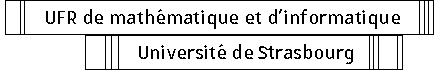
\includegraphics[width=6.5cm]{logos/logo-ufr.pdf}
  \vfill
  \vfill

  {
  \large
  \textsc {
    Master de Science, mention Informatique
    spécialité Science et Ingénierie des Réseaux, de l'Internet
    et des Systèmes
  }
  }

  \bigskip
  %\bigskip

  {\large Mémoire de projet de Master, groupe n\up{o}2}
  \vfill

  
\includegraphics[height=1.0cm]{logos/alggot.png}
  \vfill

  \medskip

  % Identité de l'auteur
  \begin{tabular}{c c c}
  {\large Adrien} &
    {\large Ludovic} &
    {\large Oussema} \\
  {\large \textsc{Roberty}} &
    {\large \textsc{Muller}} &
    {\large \textsc{Tourki}} \\
  {\small roberty@etu.unistra.fr} &
    {\small ludovic.muller2@etu.unistra.fr} &
    {\small oussema.tourki@etu.unistra.fr} \\ \hline
  {\large Govindaraj} &
    {\large Thomas} &
    {\large Gabriel} \\
  {\large \textsc{Vetrivel}} &
    {\large \textsc{Froeliger}} &
    {\large \textsc{Poittevin}} \\
  {\small govindaraj.vetrivel@etu.unistra.fr} &
    {\small thomas.froeliger@etu.unistra.fr} &
    {\small gabriel.poittevin@etu.unistra.fr}
  \end{tabular}

  \vfill

  {
  \begin{spacing}{1.4}
  \huge
  \textsc {
  \textbf {
      ChaTalK, application de télécommunications sécurisées et centralisées
  }
  }
  \end{spacing}
  }
  \vfill
  
\includegraphics[height=2.4cm]{logos/chatalk.png}
  \vfill

  {\large Projet encadré et commandité par}

  \medskip

  % Identité de l'encadrant
  {\large Julien \textsc {Montavont}}
  % Contact mail ou téléphone
  {\small montavont@unistra.fr}
  et
  % Identité de l'encadrant
  {\large Cristel \textsc {Pelsser}}
  % Contact mail ou téléphone
  {\small pelsser@unistra.fr}

  \medskip

  % Logo du client (Journalistes Sans Papiers)
  
\includegraphics[height=1.2cm]{logos/icube.png}
  \vfill
  
\includegraphics[height=1.2cm]{logos/jsp.png}

  {\small \today}
\end{center}

\cleardoublepage

% Old title page
% Ancienne page de garde
%\maketitle

\tableofcontents
\listoffigures
%\listoftables

\cleardoublepage

\begin{abstract}
  Ceci est le mémoire de projet du groupe n\up{o}2 de projet de Master de la promotion 2018-2020 du Master SIRIS de l'Université de Strasbourg.
\newline
L'objectif de ce document est de présenter le projet dans son ensemble, avec ses problématiques, les solutions qui leur ont été apportées et les difficultés rencontrées au cours de sa réalisation.
\end{abstract}

% Section Introduction
%  - présentation du projet
%  - description générale de la solution
%    - architecture
%    - technologies
\section{Introduction}


% Section Technique
%  - présentation des choix technique
%  - justification des choix
%  - regard critique sur les choix
%  - perspectives d'amélioration
%  - satisfaction des critères
\section{Technique}


% Section Solution
%  - présentation de la solution effective
%  - détails
\chapter{Solution}

La solution telle que nous l'avons conçue comprenait plusieurs
éléments que nous allons rappeler ci-dessous.

\paragraph{Tolérance aux pannes et passage à l'échelle} Grâce
à son infrasctucture basée sur Kubernetes et à son
architecture en micro-services, notre application est
aisément capable de passer à l'échelle et de supporter la
montée en charge, ainsi que de résister à la perte de
machines dans les grappes Kubernetes. Dans les pires cas, les
les fonctionnalités passent en mode dégradé. Ce mode dégradé
permet la consultation des archives de conversations et donc
de conserver une partie des activités des utilisateurs du
service.

\paragraph{Sécurité} Notre application devait garantir la
sécurité des flux de données, en particulier d'un point de
vue intégrité et confidentialité. Seuls les envoyeurs et
récepteurs des messages devaient avoir accès aux données.\\
Nous avons partiellement rempli cet objectif, des contraintes
de temps liées à nos retards nous ayant forcé à abandonner le
chiffrement des flux audiovisuels. L'authentification des
utilisateurs a néanmoins été réalisée. Une couche de sécurité
minimale basée sur SSL/TLS assure un niveau de sécurité
décent, tant que les utilisateurs du service font confiance
à l'administrateur des serveurs sur lesquels fonctionne la
solution.

\paragraph{Déploiement facile} Notre application devait
pouvoir être facilement déployée par un néophyte, sur
n'importe quelle machine de type Linux, rapidement et sans
connexion Internet. Cette tâche était d'une priorité maximale
%[[Expliquer]]

\paragraph{Temps réel} Notre application devait assurer des
conversations en temps réel entre les utilisateurs.\\
Nos tests actuels ne sont pas représentatifs d'une utilisation
réelle, mais montrent que la latence des communications
textuelles sur notre solution est imperceptible à l'humain
pour un petit nombre d'utilisateurs.

\paragraph{Interface utilisateur} Notre solution devait
proposer une interface utilisateur compatible avec un maximum
d'appareils.\\
Notre application frontale Web est utilisable sur tous les
navigateurs modernes sans modification et sans distinction
de système d'expoitation. De plus elle s'adapte à des tailles
d'écran diverses et à des appareils de puissance variée. Bien
que cette interface Web puisse être utilisée en tant
qu'application mobile, une application mobile pour Android
en Kotlin est également disponible, plus adaptée à
l'utilisation sur des téléphones intelligents.\\
Nous avons choisi une interface utilisateur épurée, en
conservant les icônograpies habituelles, afin de permettre
une meilleure expérience utilisateur et une plus grande
ergonomie.

\paragraph{Modularité} Notre solution devait permettre à un
individu déployant un serveur de choisir les capacités qu'il
souhaitait donner à celui-ci.\\
À cause des contraintes de temps, et puisque la tâche n'était
pas prioritaire, elle a été la première abandonnée totalement.
Les fonctionnalités supplémentaires audio et vidéo ont été
incluses directement dans l'application d'arrière-plan
principale et le concept de modules serveur a été laissé à
l'abandon.

\paragraph{Compatibilité et standards} Notre application
devait être compatible avec un maximum de standards et ne
pas utiliser de technologies trop peu orthodoxes.\\
Puisque l'interface utilisée est une interface Web, les quatre
systèmes d'exploitation les plus courants, Microsoft Windows,
Apple macOS, Apple iOS et Android, sont couverts tant qu'ils
possèdent un navigateur Internet à jour. De plus, les systèmes
d'exploitation GNU/Linux et BSD sont également couverts tant
qu'ils possèdent un navigateur Internet à jour. Enfin, s'il
n'existe pas d'application native pour iOS, il en existe une
pour Android.\\
D'un point de vue des standards, notre application est
accessible à des clients utilisant indifféremment de l'IPv4,
de l'IPv6 ou les deux.

\paragraph{Internationalisation} Notre application se devait
de supporter les principaux alphabets du monde et d'être
disponible à minima en Anglais.\\
Puisque tous les textes que nous utilisons sont encodés en
UTF-8, les alphabets divers sont gérés dans l'application.
L'interface que nous avons développée l'a été en Anglais et
est donc utilisable par des utilisateurs anglophones.


% Section Gestion de projet
%  - méthode de travail
%  - gestion et partage du travail
%  - outils utilisés
%  - réactivité, gestion humaine
\chapter{Gestion de projet}

% Décrire la gestion de projet
% Section Gestion de projet
%  - méthode de travail
%  - gestion et partage du travail
%  - outils utilisés
%  - réactivité, gestion humaine

\section{Organisation et commentaire général du projet}

Au départ du projet, nous avions prévu des binômes s'occupant
des tâches. Au fil du déroulement du projet, nous nous sommes
aperçus que certaines parties du projet avançaient plus vite
que d'autres, et que l'idée de binômes a changé pour confier
à chacun les tâches dans lesquelles il se sentait à l'aise.
\newline

Le suivi du projet était assuré par des réunions régulières
avec les clients / professeurs, entre une réunion par semaine
et une réunion pour deux semaines selon les périodes. Ces
réunions étaient suivies d'un compte-rendu à l'équipe projet,
durant lequel le nouveau planning était généralement présenté,
et où les tâches à venir étaient réparties entre les membres
de l'équipe.
\newline

Les membres de l'équipe étaient informés de leurs missions
via trois moyens principaux :
\begin{itemize}
  \item des \textit{issues} GitLab, avec une date, une mission et un responsable
  \item une notification écrite sur l'application de communication Discord
  \item une notification orale, généralement à la fin de la réunion de répartition des tâches
\end{itemize}
Malgré les efforts mis par le chef de projet pour notifier son
équipe des missions à réaliser, il est arrivé trop souvent
que les issues soient créées tardivement et que la
notification orale reste la seule information donnée à
l'équipe.
\newline

La plus grosse difficulté pour l'organisation de ce projet a
été de l'ordre de la communication. Gabriel a souvent été peu
réactif à officialiser par écrit les tâches à réaliser d'une
semaine sur l'autre. Le reste de l'équipe a été peu proactive,
en particulier au début, pour donner des retours sur ses
avancements et les tâches sur lesquelles elle travaillait et
comment ces tâches avançaient.

\section{Outils utilisés pour l'organisation et la gestion du projet}

\paragraph{Discord} L'outil principal utilisé pour
l'organisation et la gestion du projet a été le logiciel de
messagerie textuelle et vocale Discord. Nous l'avons choisi
car nous l'utilisons tous quotidiennement et qu'il nous
permet l'utilisation de certaines fonctionnalités pratiques
comme la création de canaux thématiques pour ne pas mélanger
les communication à propos de plusieurs tâches, ou l'épinglage
de messages pour les retrouver facilement.

\paragraph{Réunions en présentiel} Un outil très efficace que
nous avons utilisé lors de l'organisation du projet a été les
réunions en présentiel, avec autant de membres de l'équipe que
possible. Rétrospectivement, nous aurions du en faire plus
souvent. Lors de ces réunions, l'utilisation d'un tableau
blanc nous permettait de schématiser et de planifier. Ces
réunions étaient également propices à l'entraide et à la
pédagogie, permettant des explications en face à face direct.

\paragraph{Git et GitLab} Pour gérer le code source Git est
devenu un outil indispensable. Toutefois, outre cette
utilisation, la création de problèmes suivis a permis
de communiquer sur les spécification des tâches à plusieurs
reprises. Les historiques de \textit{commit} permettent plus
ou moins de voir qui a travaillé à quel moment et de détecter
les passages à vide.

\paragraph{Gantt Project} Pour créer et officialiser le
planning, l'outil Gantt Project a été utilisé, permettant de
créer simplement des diagrammes de Gantt. Ces diagrammes ont ensuite été partagés sur le dépôt GitLab pour que tous puissent les consulter.

\section{Réactivité et gestion humaine}

L'un des plus gros problèmes de ce projet a été la gestion de
la communication. D'un côté certains membres de l'équipe ont
été peu proactifs en ce qui concerne le fait d'informer les
autres de leur avancement, mais également de leurs
difficultés. Certains membres de l'équipe ont également été
peu réactifs à informer le chef du projet de leur
impossibilité temporaire à remplir leurs fonctions (maladie,
problèmes personnels grâves). D'un autre côté, le chef de
projet n'a pas été s'enquérir rapidement de l'état de ses
équipiers lorsque ceux-ci étaient absents ou ne donnaient pas
de nouvelles pendant plusieurs jours.
\newline

Ce manque de communication a posé problème pour la
redistribution des tâches auprès des autres membres de
l'équipe. Si l'informations avait été obtenue plus tôt, les
tâches non assurées auraient pu l'être par quelqu'un d'autre
et le retard aurait été mitigé.
\newline

Toutefois, lors des cinq dernières semaines du projet,
lorsqu'une tâche devait être réattribuée, elle l'a été sans
délai, pendant la période nécessaire.


% Section Évolution du planning
%  - présentation des Gantt
%  - discussion sur leur évolution et les raisons
\section{Diagrammes de Gantt, planning et évolutions}

% Section Évolution du planning
%  - présentation des Gantt
%  - discussion sur leur évolution et les raisons


% Section Timesheets
%  - discussion sur la répartition du temps
%    et de la charge de travail
%  - présentation des six timesheets (timesheets à faire)
\chapter{Emplois du temps et répartition du travail}

% Section Timesheets
%  - discussion sur la répartition du temps
%    et de la charge de travail
%  - présentation des six timesheets (timesheets à faire)

%\begin{figure}[h]
%  \caption{\label{lab} Title}
%  \includegraphics[width=15cm]{images/}
%\end{figure}

En tant que chef de projet, l'inexpérience de Gabriel
se voit également dans sa méconnaissance du concept de
\textit{timesheet} ou fiche horaire. Ce mécanisme permet
de garder une trace du temps passé par un individu sur
une tâche donnée.

N'ayant pas utilisé un logiciel dédié au suivi du temps
passé sur les tâches il est très compliqué d'estimer le
temps passé par chacun sur les tâches qui lui étaient
attribuées.

\subsection{Répartition du travail}

Dans l'équipe, les tâches ont lentement été réparties et peu de gens ont
réellement changé de fonction entre les début et la fin du projet.

\paragraph{Adrien Roberty} Adrien a d'abord été affecté la conception de
la sécurité de l'application. Plus tard dans le projet il a contribué à
l'écriture de certains services de l'arrière-plan de l'application.
Finalement il a conçu et programmé la partie communication audiovisuelle
de l'application.

\paragraph{Oussema Tourki} Oussema a été rapidement affecté à la programmation
du frontal de l'application en React JS, une technologie qu'il ne connaissait
pas et avec laquelle il beaucoup progressé depuis le début du projet. À
certains moments au milieu du projet Oussema semblait un peu embêté par ses
tâches, mais ne s'en ait jamais plaint.

\paragraph{Thomas Froeliger} Thomas a commencé le projet en travaillant en
tandem avec Adrien sur la conception de la sécurité de l'application, puis
a continué en développant en partie cette fonctionnalité. Il y a eu plusieurs
passages à vide dans le travail de Thomas, des périodes où aucune nouvelle
ne venaient de lui entre début et fin novembre en particulier.

\paragraph{Ludovic Muller} Ludovic a été un véritable pilier sur ce projet
capable de réaliser toute les tâches qu'on lui demandait, et parfois un peu
trop. Son influence a été à la fois bénéfique, car il permit de garder le
moral au mieux dans les passages difficiles, mais il semble que nous ayons
eu un peu trop tendance à nous appuyer sur lui, ce qui n'aurait peut-être pas
été le cas s'il avait été moins proactif. Il a toutefois réalisé
l'infrastructure de l'application avec brio.

\paragraph{Govindaraj Vetrivel} Govin est devenu responsable technique, car
il touchait à toutes les parties de l'application et en a rapidement compris
le fonctionnement malgré le manque de documentation, ce qui a été un atout
majeur pour aider le reste du groupe à faire fonctionner ensemble les divers
morceaux de l'application.

\paragraph{Gabriel Poittevin} Gabriel n'a pas été d'une grande aide technique,
s'étant surtout occupé de la base de données et de la gestion de projets.



% Section conclusion
%  - différences entre solution envisagée et solution effective
%  - explication des différences
%  - retour d'expérience
\chapter{Conclusion}


%\clearpage
%
%\bibliographystyle{plain}
%\bibliography{references}

\end{document}
